\documentclass[11pt,a4paper]{article}
\usepackage[T1]{fontenc}
\usepackage[utf8]{inputenc}
\usepackage{lmodern}
\usepackage[margin=24mm]{geometry}
\usepackage{amsmath,amssymb,graphicx,booktabs,array,microtype,hyperref}
\hypersetup{colorlinks=true,linkcolor=black,citecolor=blue,urlcolor=blue}
\setlength{\emergencystretch}{2em}
\title{Boundary stiffness, radion residues and fixed-action length selection in a five-dimensional interval}
\author{Hicham Boufourou}
\date{7 September 2026}
\begin{document}
\maketitle
\begin{abstract}
We calculate the radion mass and its canonically normalized same-boundary residue in a reflection-symmetric five-dimensional interval with a canonical scalar, a convex quadratic bulk potential and finite-stiffness quadratic boundary potentials. In a reconstructed family at fixed dimensionless bulk mass and stiffness, both leading weak-backreaction coefficients have closed forms: increasing stiffness raises the mass coefficient and lowers the positive residue correction. Their affine and rigid limits bound a mass-residue consistency coefficient without requiring an absolute compactification scale. Independently, fixed dimensional action parameters select a unique scalar endpoint, while a flat gravitational solution also requires the compatible boundary tension. Positive massive-mode forms are supplemented by an explicit null-shell analysis of the complete junctions and presymplectic form. Profile quadrature, an independent spectral discretization and background-event calculations test the results. A local tension detuning reproduces the expected unsuppressed vacuum-energy response. These are conditional results of a specified classical model; no ultraviolet completion, absolute radius or observational viability is inferred.
\end{abstract}
\section*{1. Introduction}
A compact extra dimension requires both a mechanism that fixes its proper length and a calculation of the interactions of its light gravitational scalar. Bulk-scalar stabilization and backreacted scalar-gravity backgrounds are established tools \cite{ref1,ref2}. The dark-dimension scenario provides a separate motivation for studying a light compact direction \cite{ref12}, but it does not specify the stabilizer or boundary coefficients of the model studied here. In one particular Casimir realization, Cui and Ning find a radion that is too light for the constraints they consider \cite{ref15}. This motivates studying masses and couplings together; it is not an exclusion theorem for all Casimir models or evidence for the present alternative.

We examine a physical interval with a canonical scalar, a positive constant plus a convex quadratic bulk potential, and quadratic boundary potentials of finite stiffness. Its reflection-symmetric branch has an odd scalar and a warp factor with an interior maximum. The interval formulation \cite{ref13}, scalar perturbation equations \cite{ref3}, canonical normalization \cite{ref4} and spectral criteria \cite{ref5,ref6,ref14} are established methods. Earlier stabilized geometries include equal endpoint warp factors \cite{ref7} and genuinely reflection-symmetric constructions \cite{ref8}; these properties are not equivalent. Finite brane potentials and their modified scalar products have also been studied analytically and numerically \cite{ref23}.

The main calculation here is the explicit leading same-boundary radion residue for this convex, symmetric model, together with its stiffness bounds and its relation to the radion mass. Conditional fixed-action length selection and local tension-response benchmarks specify the backgrounds on which that calculation is used. Monotonicity of scalar masses with boundary stiffness, endpoint corrections to spectral products and the unsuppressed vacuum response have precedents \cite{ref2,ref6,ref9,ref23}; they are not asserted as new general principles. Section 9 compares the potentials, approximations and observables of the closest works.

Two parameter experiments will be kept distinct. Determining length at fixed dimensional action is a boundary-value problem. Comparing stiffnesses on one prescribed background instead requires reconstructing boundary minima and constants, and compares different actions \cite{ref6}. Section 3 treats the first problem; Sections 4-6 calculate spectra and residues in the second. Section 7 detunes a compatible flat solution, and Section 8 defines the corresponding exchange observable. The null momentum shell and its boundary domain are proved in Appendix B. Matter is in its vacuum throughout the stability analysis.

\section*{2. Action, dimensions and boundary data}
Use signature (-++++), natural units and a single physical interval 0\ensuremath{\leq}y\ensuremath{\leq}L. Write B=M\ensuremath{{}_{5}}\ensuremath{{}^{3}}>0. The Gibbons-Hawking-York term has coefficient B and the outward normal signs are \ensuremath{\eta}\ensuremath{{}_{0}}=-1 and \ensuremath{\eta}L=+1. There is no second bulk copy. Matter couples minimally to the induced metric at the left boundary.

\begin{equation}
S=\int_0^Ldy\int d^4x\sqrt{-g}\left[\frac{B}{2}{\cal R}_5-\frac12(\partial\sigma)^2-V(\sigma)\right]\tag{1a}
\end{equation}
\begin{equation}
\quad+B\int_{\partial M}d^4x\sqrt{-\gamma}\,K-\sum_i\int_i d^4x\sqrt{-\gamma}\,U_i(\sigma)+S_m[\gamma_0].\tag{1b}
\end{equation}
\begin{equation}
V=\Lambda_5+\frac12\mu^2\sigma^2,\quad U_0=\tau+\lambda(\sigma+v)^2,\quad U_L=\tau+\lambda(\sigma-v)^2.\tag{2}
\end{equation}
Throughout the main branch \ensuremath{\mu},\ensuremath{\lambda},v are positive. Reflection y\ensuremath{\to}L-y combined with \ensuremath{\sigma}\ensuremath{\to}-\ensuremath{\sigma} exchanges the boundaries. The absence of scalar or Einstein kinetic terms on the boundaries and of direct matter-stabilizer couplings is part of the definition of this classical truncation. These operators are not claimed to be forbidden by a quantum symmetry.

\begin{table}[htbp]
\centering\small
\begin{tabular}{ccc}
\toprule
Quantity & Mass dimension & Role\\
\midrule
B=M\ensuremath{{}_{5}}\ensuremath{{}^{3}} & 3 & Gravitational coefficient\\
\ensuremath{\mu}, \ensuremath{\lambda} & 1 & Bulk mass, boundary stiffness\\
\ensuremath{\sigma}, v & 3/2 & Scalar, preferred boundary value\\
\ensuremath{\Lambda}\ensuremath{{}_{5}} & 5 & Bulk constant\\
\ensuremath{\tau}, \ensuremath{U_i} & 4 & Boundary vacuum energies\\
L, R\ensuremath{{}_{0}}=L/\ensuremath{\pi} & -1 & Proper length, conventional radius\\
\bottomrule
\end{tabular}
\caption{Independent dimensional inputs and geometric outputs. A choice of units does not determine a dimensional scale.}
\end{table}
For \ensuremath{ds^2=e^{2A}\eta_{\mu\nu}\,dx^\mu dx^\nu+dy^2}, the exact flat-slice equations and junctions are

\begin{equation}
A^{\prime\prime}=-\frac{\sigma^{\prime2}}{3B},\quad \sigma^{\prime\prime}=\mu^2\sigma-4A^\prime\sigma^\prime,\quad 6B A^{\prime2}=\frac{\sigma^{\prime2}}{2}-\frac{\mu^2\sigma^2}{2}-\Lambda_5,\tag{3a}
\end{equation}
\begin{equation}
U_i(\sigma_i)=3\eta_i B A_i^\prime,\qquad \eta_i\sigma_i^\prime=-U_i^\prime(\sigma_i).\tag{3b}
\end{equation}
The junction fixes the total value \ensuremath{U_i} on the solution, not only the constant \ensuremath{\tau}. In the symmetric branch the two total values are negative. A negative total boundary energy is not interchangeable with a negative kinetic norm; the latter is computed below. No microscopic realization of the boundaries is supplied.

\section*{3. Length selection with fixed dimensional parameters}
Place t=0 at the reflection center. Symmetry fixes \ensuremath{\sigma}(0)=A\ensuremath{{}^{\prime}}(0)=0, and the Einstein constraint fixes \ensuremath{\sigma^{\prime}(0)=\sqrt{2\Lambda_5}}. Set A(0)=0 temporarily. With \ensuremath{\mu},\ensuremath{\lambda},v,\ensuremath{\Lambda}\ensuremath{{}_{5}},B given, no central slope remains available to tune an arbitrarily selected length. The right scalar boundary is the first positive zero of

\begin{equation}
F(t)=\sigma^\prime(t)+2\lambda\sigma(t)-2\lambda v,\qquad L=2t_* .\tag{4}
\end{equation}
For t>0 on a regular solution, \ensuremath{\sigma}\ensuremath{{}^{\prime}}>0, \ensuremath{\sigma}>0 and A\ensuremath{{}^{\prime}}<0. Consequently \ensuremath{\sigma}\ensuremath{{}^{\prime\prime}}>0 and F\ensuremath{{}^{\prime}}=\ensuremath{\sigma}\ensuremath{{}^{\prime\prime}}+2\ensuremath{\lambda}\ensuremath{\sigma}\ensuremath{{}^{\prime}}>0. If F(0)<0, then before a root one has \ensuremath{\sigma}<v and \ensuremath{\sigma}\ensuremath{{}^{\prime}}<2\ensuremath{\lambda}v. These bounds also bound A\ensuremath{{}^{\prime}} on any finite segment and prevent a finite-time blow-up before the root. Since \ensuremath{\sigma^{\prime}\geq\sqrt{2\Lambda_5}}, F(t) is bounded below by \ensuremath{\sqrt{2\Lambda_5}+2\lambda\sqrt{2\Lambda_5}\,t-2\lambda v}; hence it must reach zero in finite time. The root is unique. If F(0)\ensuremath{\geq}0, strict monotonicity excludes a positive root. Thus the scalar boundary exists uniquely precisely when

\begin{equation}
0<\Lambda_5<2\lambda^2v^2.\tag{5}
\end{equation}
This statement selects the scalar endpoint, not an arbitrary flat solution of the complete action. The remaining metric junction requires the independent constant of the action to equal

\begin{equation}
\tau_{\rm flat}=3B A_b^\prime-\lambda(\sigma_b-v)^2.\tag{6}
\end{equation}
If \ensuremath{\tau} has another value, the selected configuration is not a Minkowski solution of that action. Section 7 solves a local curved continuation with \ensuremath{\tau} supplied independently. This separates a compatibility condition from a prediction and displays the vacuum-energy tuning directly.

The scalar can also be integrated exactly on a flat fixed metric. This gives the leading weak-backreaction radion potential, not an exact gravitational solution. With u=\ensuremath{\mu}L/2 and a=2\ensuremath{\lambda}/\ensuremath{\mu},

\begin{equation}
q(L)=\frac{2\lambda v}{1+a\tanh u},\quad \sigma(y)=\frac{q(L)\sinh[\mu(y-L/2)]}{\mu\cosh u},\tag{7a}
\end{equation}
\begin{equation}
E_\sigma(L)=\frac{2\lambda v^2}{1+a\tanh u},\qquad V_J=\Lambda_5L+2\tau+E_\sigma(L).\tag{7b}
\end{equation}
The energy follows by integrating the bulk term to [\ensuremath{\sigma}\ensuremath{\sigma}\ensuremath{{}^{\prime}}]/2 and adding both boundary quadratics. In particular q changes with L at fixed action. Defining \ensuremath{H=\cosh u+a\sinh u} and \ensuremath{K=\sinh u+a\cosh u} gives \ensuremath{E_\sigma^{\prime}=-2\lambda^2v^2/H^2} and \ensuremath{E_\sigma^{\prime\prime}=2\mu\lambda^2v^2K/H^3>0}. The tuned Minkowski extremum satisfies \ensuremath{V_J=V_J^{\prime}=0}. For \ensuremath{\zeta=\sqrt{2}\lambda v/\sqrt{\Lambda_5}>1} its length is

\begin{equation}
L_{\rm flat}=\frac{2}{\mu}\log\left[\frac{\zeta+\sqrt{\zeta^2+a^2-1}}{1+a}\right],\qquad 2\tau=-\Lambda_5L_{\rm flat}-E_\sigma(L_{\rm flat}).\tag{8}
\end{equation}
The positive logarithm branch is physical. At its flat-metric extremum H=\ensuremath{\zeta}, the central derivative of (7a) is \ensuremath{2\lambda v/H=\sqrt{2\Lambda_5}}, exactly the slope fixed by the Einstein constraint for the backreacted problem. Thus the comparison uses identical central scalar data. The term -4A\ensuremath{{}^{\prime}}\ensuremath{\sigma}\ensuremath{{}^{\prime}} is positive away from the center and increases both \ensuremath{\sigma} and \ensuremath{\sigma}\ensuremath{{}^{\prime}} relative to the flat-metric solution. The exact scalar event is reached earlier, giving 0<L<\ensuremath{L_{\mathrm{flat}}} for finite B. Compatible boundary tensions need not coincide in the two approximations. This comparison fixes \ensuremath{\mu},\ensuremath{\lambda},v,\ensuremath{\Lambda}\ensuremath{{}_{5}},B; it is not the fixed-background scan of Section 5.

The Einstein-frame potential is \ensuremath{V_E=(L_{\mathrm{ref}}/L)^2V_J} at leading backreaction, with canonical length field \ensuremath{\sqrt{3/2}\,M_4\ln(L/L_{\mathrm{ref}})}. At a Minkowski extremum, \ensuremath{V_J=V_J^{\prime}=0} removes additional Weyl terms from its Hessian. For \ensuremath{L_{\mathrm{ref}}=L_*}, \ensuremath{M_4^2=BL_*},

\begin{equation}
m_r^2=\frac{2L_*^2}{3M_4^2}E_\sigma^{\prime\prime}(L_*)>0.\tag{9}
\end{equation}
This Hessian reproduces the leading coefficient found independently from fluctuations in Section 5. For the exact background, z=\ensuremath{\mu}t, s=\ensuremath{\sigma}/v and \ensuremath{\beta}=v\ensuremath{{}^{2}}/B give

\begin{equation}
A_{zz}=-\frac{\beta}{3}(s_z)^2,\quad s_{zz}=s-4A_zs_z,\quad s(0)=A_z(0)=0,\quad s_z(0)=a/\zeta.\tag{9b}
\end{equation}
If \ensuremath{z_*(a,\zeta,\beta)} is the scalar boundary event, \ensuremath{R_0=2z_*/(\pi\mu)}. The explicit factor 1/\ensuremath{\mu} shows why dimensional input remains necessary.

Having selected a background and its compatible tension, the next question is whether its fluctuations define a regular positive-norm spectrum. The spectral calculation also fixes the normalization required for the radion residue; a minimum of a reduced length potential alone would not determine that residue.

\section*{4. Scalar spectrum, physical norm and boundary stiffness}
First consider nonzero four-dimensional momentum invariant in a straight-boundary scalar gauge: \ensuremath{ds^2=e^{2A+2F}\eta_{\mu\nu}\,dx^\mu dx^\nu+e^{-4F}dy^2}, \ensuremath{F=f(y)\chi(x)}, \ensuremath{\delta\sigma=s(y)\chi(x)}, with \ensuremath{(\Box_4-m^2)\chi=0}. The null shell p\ensuremath{{}^{2}}=0, \ensuremath{p_\mu}\ensuremath{\ne}0 requires a separate reconstruction because the usual scalar and tensor projections become dependent there. Appendix B supplies that reconstruction and establishes when the zero-shift straight-boundary representative is admissible. The massive scalar constraint and regular bulk equation are \cite{ref3,ref4}

\begin{equation}
3B(f^\prime+2A^\prime f)+\sigma^\prime s=0,\qquad W=\frac{\sigma^{\prime\prime}}{\sigma^\prime},\tag{10}
\end{equation}
\begin{equation}
f^{\prime\prime}+(2A^\prime-2W)f^\prime+(4A^{\prime\prime}-4A^\prime W+m^2e^{-2A})f=0.\tag{11}
\end{equation}
No division by A\ensuremath{{}^{\prime}} occurs, so the interior maximum of A is regular. Nonzero \ensuremath{\sigma}\ensuremath{{}^{\prime}} is essential and holds on the branch of Section 3. Perturbing the scalar junction, including the normal metric perturbation, gives \ensuremath{s_i^{\prime}+2\sigma_i^{\prime}f_i+\eta_iU_i^{\prime\prime}s_i=0}. With \ensuremath{D_i=W_i+2\eta_i\lambda} this becomes

\begin{equation}
D_i(f_i^\prime+2A_i^\prime f_i)=m^2e^{-2A_i}f_i.\tag{12}
\end{equation}
The factor two is fixed by U=\ensuremath{\lambda}(\ensuremath{\sigma}-v\ensuremath{{}_{i}})\ensuremath{{}^{2}}. Set g=e\ensuremath{{}^{2A}}f and define the positive bulk coefficients

\begin{equation}
p=\frac{e^{-2A}}{\sigma^{\prime2}},\quad w=\frac{e^{-4A}}{\sigma^{\prime2}},\quad Q=\frac{2e^{-2A}}{3B},\quad -(pg^\prime)^\prime+Qg=m^2wg.\tag{13}
\end{equation}
\begin{equation}
{\cal K}[g]=\int_0^L(p|g^\prime|^2+Q|g|^2)dy=m^2{\cal D}[g],\tag{14a}
\end{equation}
\begin{equation}
{\cal D}[g]=\int_0^Lw|g|^2dy+\sum_i\frac{w_i|g_i|^2}{\eta_iW_i+2\lambda}.\tag{14b}
\end{equation}
On the regular symmetric branch, \ensuremath{\sigma}\ensuremath{{}^{\prime}}>0 and \ensuremath{\sigma}\ensuremath{{}^{\prime\prime}}=\ensuremath{\mu}\ensuremath{{}^{2}}\ensuremath{\sigma}-4A\ensuremath{{}^{\prime}}\ensuremath{\sigma}\ensuremath{{}^{\prime}}>0 to the right of the center follow analytically from the positive central slope, \ensuremath{\sigma}>0 and A\ensuremath{{}^{\prime}}<0. Reflection gives \ensuremath{W_0}<0<\ensuremath{W_L}. Hence \ensuremath{\eta}\ensuremath{{}_{i}}W\ensuremath{{}_{i}}+2\ensuremath{\lambda}>0 at both endpoints for positive stiffness. The forms are strictly positive for any nonzero mode; the conjugated identity establishes real, strictly positive scalar eigenvalues. These are specialized instances of established criteria \cite{ref5,ref6,ref23}. Zeros of \ensuremath{\sigma}\ensuremath{{}^{\prime}} or endpoint denominators, added boundary kinetic operators and curved slices require separate treatment.

At a fixed background, increasing stiffness decreases the boundary contribution to D while K is unchanged. The min-max principle therefore makes every ordered scalar squared mass nondecreasing, as in the general analysis of \cite{ref6}. The rigid limit has no boundary spectral weights and imposes g\ensuremath{{}_{i}}\ensuremath{{}^{\prime}}=0; finite \ensuremath{\lambda}L=20 is not that limit. Holding the background fixed requires \ensuremath{v_i=\sigma_i+\eta_iq_i/(2\lambda)} and \ensuremath{\tau_i=3\eta_iBA_i^{\prime}-q_i^2/(4\lambda)}, so this experiment reconstructs the action. The affine action \ensuremath{U_i}=T\ensuremath{{}_{i}}+J\ensuremath{{}_{i}}\ensuremath{\sigma} is a separate comparison family; its fixed-background \ensuremath{\lambda}\ensuremath{\to}0 limit requires divergent minima and subtracted constants.

The generalized spectral product D is not the canonical kinetic normalization. The ADM gravitational and scalar terms yield the two contributions to (15). In this fixed-boundary, zero-shift representative the potentials carry no spacetime derivatives and the GHY corner contribution vanishes. This gauge-specific simplification is not used for the null-shell analysis in Appendix B, which retains the mixed metric perturbation and all corners. With A(0)=A(L)=0 and I=\ensuremath{\int}e\ensuremath{{}^{2A}}dy,

\begin{equation}
N_f=\int_0^Le^{2A}\left(3B f^2+\frac{s^2}{2}\right)dy=\frac{9B^2}{2}{\cal K}[g],\qquad Z_f=2N_f.\tag{15}
\end{equation}
\begin{equation}
M_4^2=BI,\qquad g_f=\frac{f(0)}{\sqrt{2N_f}},\qquad \alpha_f=2M_4^2g_f^2=\frac{BI f(0)^2}{N_f}.\tag{16}
\end{equation}
The Yukawa residue is measured relative to the massless tensor exchange \ensuremath{G_T=1/(8\pi M_4^2)}. It is independent of profile normalization and tends to 1/3 for the unstabilized flat radion. Tensor modes obey \ensuremath{-(e^{4A}h^{\prime})^{\prime}=m_T^2e^{2A}h} with Neumann endpoints; integration gives \ensuremath{m_T^2\int e^{2A}|h|^2dy=\int e^{4A}|h^{\prime}|^2dy\geq0}. The only tensor zero mode is constant on the connected interval \cite{ref14}.

For p\ensuremath{{}^{2}}\ensuremath{\ne}0 there is no additional propagating vector tower. In Gaussian normal bulk coordinates, retaining boundary embeddings, a transverse vector perturbation has \ensuremath{h_{\mu\nu}=\partial_\mu V_\nu+\partial_\nu V_\mu} and \ensuremath{\partial^\mu V_\mu=0}. The mixed Einstein constraint gives \ensuremath{\Box_4 V_\mu^{\prime}=0}; thus \ensuremath{V_\mu}\ensuremath{{}^{\prime}}=0, and a residual tangential diffeomorphism removes it. The massive four-dimensional transverse-traceless tensor already contains five spin-two polarizations. Its helicity-one components must not be counted again as a separate vector field. For positive mass, the rest-frame spatial trace-free polarization tensor has positive kinetic norm.

The complete null-shell calculation in Appendix B imposes both scalar and anisotropic metric junctions on a regular null basis. For q=\ensuremath{\sigma}\ensuremath{{}_{0}}\ensuremath{{}^{\prime}} nonzero and \ensuremath{D_i}=W\ensuremath{{}_{i}}+\ensuremath{\eta}\ensuremath{{}_{i}}\ensuremath{U_i}\ensuremath{{}^{\prime\prime}} nonzero, the scalar/longitudinal null solutions reduce to diffeomorphisms with their boundary embedding transformations. Two positive-norm massless graviton polarizations remain. In particular, a formal null profile with negative extended form N=-3BI is outside the full Israel boundary domain; it is not a physical ghost. These results give linear propagative stability of the declared regular flat branch. They do not extend to static \ensuremath{p_\mu}=0 perturbations, occupied matter with backreaction, nonlinear dynamics or quantum corrections.

\section*{5. Closed mass and coupling coefficients at finite stiffness}
For the symmetric reconstructed family, fix x=\ensuremath{\mu}L>0 and equal \ensuremath{\hat{\lambda}}=\ensuremath{\lambda}L\ensuremath{\geq}0 as \ensuremath{\epsilon=qL/\sqrt{12B}} tends to zero; here \ensuremath{q=\sigma^{\prime}(0)=\sigma^{\prime}(L)} is the exact endpoint derivative. Use dimensionless coordinates \ensuremath{x^\mu/L} and y/L, and stabilizer \ensuremath{\sigma/\sqrt{B}}, and suppress hats on the reduced fields. The overall factor BL\ensuremath{{}^{3}} in the rescaled action does not affect the classical profile equations and is not set to one physically. Put t=y/L-1/2, C=cosh\ensuremath{{}^{2}}(x/2), T=tanh(x/2), S=sinh x and d=xT+2\ensuremath{\hat{\lambda}}. Derivatives in (17)-(20) refer to t. The expansions are \ensuremath{\sigma}\ensuremath{{}^{\prime}}=\ensuremath{\epsilon}v\ensuremath{{}_{1}}+O(\ensuremath{\epsilon}\ensuremath{{}^{3}}), A=\ensuremath{\epsilon}\ensuremath{{}^{2}}a\ensuremath{{}_{2}}+O(\ensuremath{\epsilon}\ensuremath{{}^{4}}), f=1+\ensuremath{\epsilon}\ensuremath{{}^{2}}f\ensuremath{{}_{2}}+O(\ensuremath{\epsilon}\ensuremath{{}^{4}}), with f\ensuremath{{}_{2}}(0)=0 at the midpoint.

\begin{equation}
v_1=\sqrt{12/C}\cosh(xt),\quad a_2^\prime=-\frac{2t+\sinh(2xt)/x}{C}.\tag{17}
\end{equation}
\begin{equation}
b=f_2^\prime+2a_2^\prime=\frac{8t\cosh^2(xt)}{C}-\frac{\kappa\sinh(2xt)}{2x},\quad d\,b(1/2)=\kappa.\tag{18}
\end{equation}
\begin{equation}
m_r^2L^2=\kappa\epsilon^2+O(\epsilon^4),\qquad \kappa(x,\widehat\lambda)=\frac{4d}{1+d\sinh(x)/(2x)}.\tag{19}
\end{equation}
Equation (19) follows by imposing the perturbed boundary condition on the bulk solution. Substitution of the flat scalar profile into (9) gives the same coefficient with \ensuremath{\hat{\lambda}}=\ensuremath{\lambda}L*: the fixed-action potential and the mode calculation are independent routes to this order. The remaining profiles are

\begin{equation}
f_2(t)=\frac{4t^2+2t\sinh(2xt)/x}{C}-\frac{\kappa[\cosh(2xt)-1]}{4x^2},\qquad s_1=-\frac{3b}{v_1}.\tag{20}
\end{equation}
Expanding the physical residue (16), the explicit Planck-volume correction cancels between numerator and denominator, as shown before (A1). With brackets denoting full-interval averaging,

\begin{equation}
3\alpha_r-1=c_\alpha\epsilon^2+O(\epsilon^4),\quad c_\alpha=2[f_2(1/2)-\langle f_2\rangle]-\frac{\langle s_1^2\rangle}{6}.\tag{21}
\end{equation}
The elementary integrals in Appendix A cancel every term linear in \ensuremath{\kappa}. They give the finite-stiffness expression

\begin{equation}
c_\alpha(x,\widehat\lambda)=\frac{1+S/x}{C}-\frac{C\kappa(x,\widehat\lambda)^2}{16x^2}(S/x-1).\tag{22}
\end{equation}
For fixed x>0, \ensuremath{\kappa} increases strictly with \ensuremath{\hat{\lambda}} while S/x>1. Thus \ensuremath{c_\alpha} decreases with \ensuremath{\hat{\lambda}}. Its affine and rigid endpoints simplify to

\begin{equation}
c_0=\frac{1+T^2+2T/x}{C},\qquad c_\infty=\frac{4[\cosh x-\sinh(x)/x]}{\sinh^2x},\qquad 0<c_\infty\le c_\alpha\le c_0.\tag{23}
\end{equation}
The strict lower bound follows because x cosh x-sinh x has derivative x sinh x>0 and vanishes at x=0. It is pointwise in x: \ensuremath{c_\infty} tends to zero for large x, so there is no uniform positive lower bound such as 1/3 on \ensuremath{c_\alpha}. The quantity approaching 1/3 in the flat unstabilized limit is \ensuremath{\alpha_r}, not \ensuremath{c_\alpha}. Increasing stiffness raises the leading mass coefficient and lowers the leading residue correction. These statements concern the fixed-x weak-backreaction expansion and give no all-orders monotonicity or uniform error estimate in degenerate limits.

\begin{table}[htbp]
\centering\small
\begin{tabular}{ccc}
\toprule
\ensuremath{\hat{\lambda}} & \ensuremath{\kappa} & \ensuremath{c_\alpha}\\
\midrule
0 & 2.558800034 & 0.983420240\\
1 & 3.359794733 & 0.839948683\\
20 & 4.297387689 & 0.622678119\\
rigid & 4.411529036 & 0.592594873\\
\bottomrule
\end{tabular}
\caption{Closed weak-backreaction coefficients at x=2; no dimensional radius is used.}
\end{table}
Eliminating \ensuremath{\epsilon} gives a relation between measurable outputs. Since the first massive tensor mode has \ensuremath{m_{T,1}L=\pi+O(\epsilon^2)},

\begin{equation}
3\alpha_r-1=\frac{\pi^2c_\alpha}{\kappa}\left(\frac{m_r}{m_{T,1}}\right)^2+O(\epsilon^4).\tag{24}
\end{equation}
A useful corollary removes the unknown stiffness from the leading consistency coefficient while retaining x. Define \ensuremath{\mathcal C_{\alpha m}=\pi^2c_\alpha/\kappa}. Since \ensuremath{c_\alpha}>0 decreases and \ensuremath{\kappa}>0 increases with stiffness, \ensuremath{\mathcal C_{\alpha m}} decreases strictly. Substitution of the endpoints in (23) gives

\begin{equation}
\frac{\pi^2}{2x}\left(\coth x-\frac1x\right)\leq {\cal C}_{\alpha m}\leq\frac{\pi^2}{2x}\left(\coth x+\frac1x\right).\tag{24b}
\end{equation}
The width of this coefficient interval is \ensuremath{\pi}\ensuremath{{}^{2}}/x\ensuremath{{}^{2}}. Equation (24) retains its O(\ensuremath{\epsilon}\ensuremath{{}^{4}}) remainder; dividing it by the squared mass ratio leaves an O(\ensuremath{\epsilon}\ensuremath{{}^{2}}) error for the inferred coefficient at fixed x. Thus (24b) bounds the leading coefficient, not an exact finite-amplitude observable. It is an algebraic corollary of (19) and (22), not an independent stabilization principle.

This relation removes the absolute length but retains x and \ensuremath{\hat{\lambda}} as shape parameters. It is therefore a conditional consistency relation rather than a parameter-free prediction of R. Its coefficients and their interpretation extend the separate affine control without silently reusing an affine boundary condition in the quadratic model.

\begin{figure}[htbp]
\centering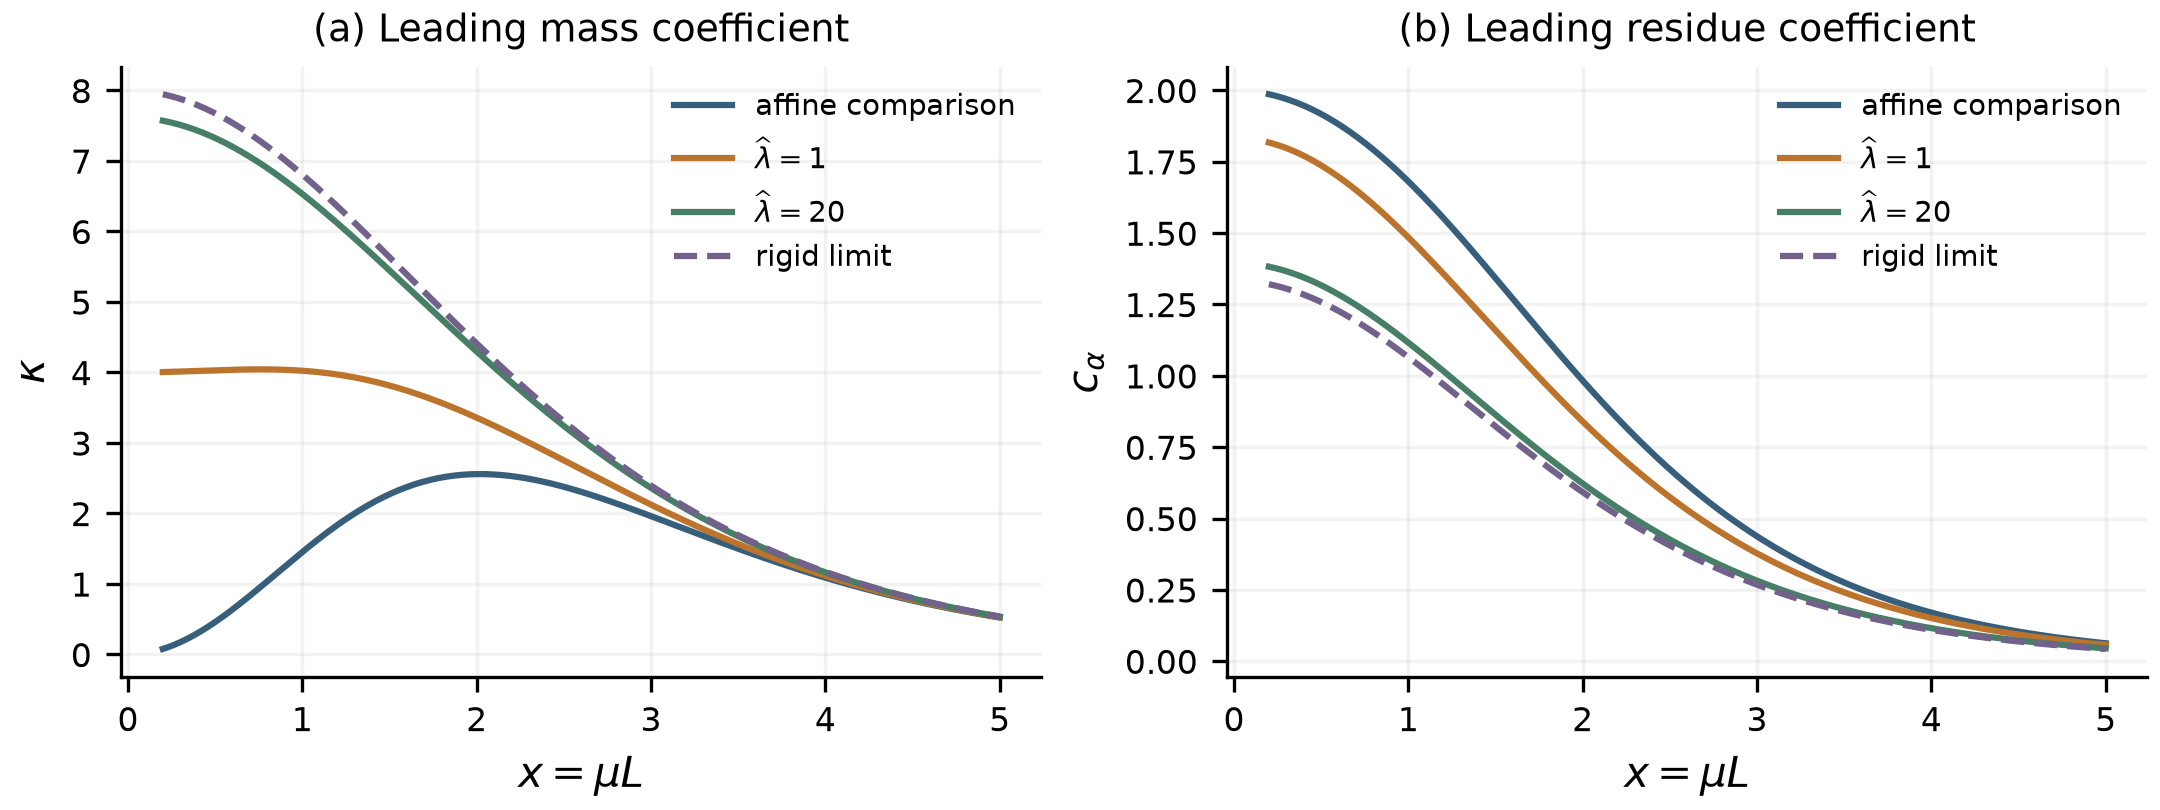
\includegraphics[width=\linewidth]{figures/finite_stiffness.png}
\caption{Leading coefficients at fixed dimensionless boundary stiffness. Increasing stiffness raises the mass coefficient and lowers the positive residue coefficient. Dashed curves refer to the limiting rigid boundary problem.}
\end{figure}
\section*{6. Finite-backreaction results and numerical controls}
The dimensionless background is integrated from the midpoint and reconstructed at x=2 for \ensuremath{\epsilon}=0.1,0.3,0.53. A Legendre-Galerkin method solves the positive generalized eigenproblem on the full interval, with 20,32,48 basis functions and 256,384,512 Gauss nodes. Independent step refinements of the background and spectral resolutions are recorded. All three retained scalar modes use positive integrals for their canonical norms. The light eigenvalue is additionally stabilized by a Schur-complement calculation in the small-\ensuremath{\epsilon} runs, where subtractive cancellation can otherwise obscure the coefficient.

\begin{table}[htbp]
\centering\small
\begin{tabular}{ccccc}
\toprule
\ensuremath{\epsilon} & \ensuremath{\hat{\lambda}} & \ensuremath{m_r} L & \ensuremath{\alpha_r} & 1/(\ensuremath{m_r} L)\\
\midrule
0.10 & 0 & 0.160208 & 0.336569 & 6.241887\\
0.10 & 1 & 0.182819 & 0.336099 & 5.469890\\
0.10 & 20 & 0.206387 & 0.335382 & 4.845259\\
0.10 & rigid & 0.209090 & 0.335283 & 4.782621\\
0.30 & 0 & 0.483691 & 0.359838 & 2.067436\\
0.30 & 1 & 0.537838 & 0.356075 & 1.859298\\
0.30 & 20 & 0.599671 & 0.350135 & 1.667580\\
0.30 & rigid & 0.607110 & 0.349286 & 1.647147\\
0.53 & 0 & 0.850124 & 0.402267 & 1.176299\\
0.53 & 1 & 0.913273 & 0.393031 & 1.094963\\
0.53 & 20 & 0.997569 & 0.377353 & 1.002437\\
0.53 & rigid & 1.008673 & 0.374981 & 0.991401\\
\bottomrule
\end{tabular}
\caption{Radion masses, residues and dimensionless Compton ranges. Every \ensuremath{\epsilon} and stiffness row has reconstructed action constants; the rigid row is a limiting boundary problem. No dimensional radius is chosen.}
\end{table}
At \ensuremath{\epsilon}=0.3 the four stiffnesses agree with the Richardson-extrapolated estimates from the earlier piecewise-linear finite-element spectral calculation to relative differences below 1.4\ensuremath{\times}10\ensuremath{{}^{-11}} for the compared radion masses and residues. The older finite-element data have their own mesh-refinement record. Agreement between discretizations checks the spectrum of the declared model; neither method certifies an ultraviolet completion or an exhaustive tower. Positivity follows from Section 4, not from finding only positive numerical roots.

The new weak-coefficient calculation also integrates the unsimplified profiles of (20)-(21) with two Simpson resolutions at 35 (x,\ensuremath{\hat{\lambda}}) points. The largest difference from (22) is below 4.7\ensuremath{\times}10\ensuremath{{}^{-14}}. Separate spectral runs at \ensuremath{\epsilon}=0.02,0.01,0.005 approach the finite-stiffness coefficients without using those coefficients in the eigensolver. For \ensuremath{\hat{\lambda}}=1, the finite-\ensuremath{\epsilon} estimate \ensuremath{(3\alpha_r-1)/\epsilon^2} changes from approximately 0.839529 to 0.839922, approaching 0.839949; for \ensuremath{\hat{\lambda}}=20 it changes from 0.622354 to 0.622658, approaching 0.622678. These are numerical convergence diagnostics, not uncertainties in physical parameters.

The benchmark family changes the total boundary energies with \ensuremath{\epsilon}. In reduced variables U\ensuremath{{}_{i}}L/B, both endpoint energies are negative. The dimensional inputs are reconstructed for every row. Increasing stiffness at a fixed background leaves \ensuremath{U_i} fixed while changing \ensuremath{\tau}\ensuremath{{}_{i}} and v\ensuremath{{}_{i}}. Table 3 therefore compares specified models; it is not a one-parameter evolution at fixed microscopic action.

\section*{7. Curvature response when the tension is an input}
To complete the background boundary-value problem near a compatible flat solution, allow maximally symmetric four-dimensional slices with scalar curvature R\ensuremath{{}_{4}}=12h. The signed parameter h is negative for anti-de Sitter slices. With A=0 at the center during the integration, the equations are

\begin{equation}
A^{\prime\prime}=-\frac{\sigma^{\prime2}}{3B}-he^{-2A},\qquad \sigma^{\prime\prime}=\mu^2\sigma-4A^\prime\sigma^\prime,\tag{25a}
\end{equation}
\begin{equation}
6B(A^{\prime2}-he^{-2A})=\frac{\sigma^{\prime2}}{2}-\frac{\mu^2\sigma^2}{2}-\Lambda_5,\quad \sigma_c^{\prime2}=2\Lambda_5-12Bh.\tag{25b}
\end{equation}
We continue a compatible flat solution in a neighborhood of h=0 where the background remains regular and the positive scalar boundary event is transverse. The central slope requires \ensuremath{h<\Lambda_5/(6B)}; on this branch the initial event value must also be negative, requiring \ensuremath{h>(\Lambda_5-2\lambda^2v^2)/(6B)}. These central inequalities do not replace regularity and event checks. For each admissible local trial the scalar event selects the endpoint and the metric junction defines \ensuremath{T(h)=3BA_b^{\prime}-\lambda(\sigma_b-v)^2}. We solve \ensuremath{T(h)=\tau_{\mathrm{input}}} at fixed \ensuremath{\mu},\ensuremath{\lambda},v,\ensuremath{\Lambda}\ensuremath{{}_{5}},B. The brane curvature is \ensuremath{h_b=h e^{-2A_b}}, and \ensuremath{M_4^2=B\int e^{2A-2A_b}dy}.

\begin{equation}
\left.\frac{d h_b}{d\tau}\right|_{\rm flat}=\frac{2}{3M_{4,0}^2},\qquad h_b=\frac{2\delta\tau}{3M_{4,0}^2}+O(\delta\tau^2).\tag{26}
\end{equation}
The derivative in (26) is an exact first-order identity at the compatible flat solution of this classical action. Using its linear term at nonzero detuning is an approximation with the displayed quadratic remainder; no finite-detuning linear law is assumed.

Here \ensuremath{\delta}\ensuremath{\tau} is the same additive variation on each boundary. At the flat background, both induced metrics have unit warp factor in brane units. The first variation of the on-shell four-dimensional vacuum energy is therefore 2\ensuremath{\delta}\ensuremath{\tau}; the stationary field and length variations do not contribute at first order. The four-dimensional Einstein equation gives (26). Equivalently, differentiating the bulk equations and the moving event reproduces this coefficient. Its nonzero value yields a local invertible map by the implicit-function theorem at the regular branch point. The general fact that stabilization does not suppress the response to added vacuum energy has direct precedents \cite{ref2,ref9}; the calculation here specializes and checks it for this non-AdS symmetric interval.

Twelve nonzero detunings near three flat reference backgrounds were solved, with two integration resolutions and one independent bisection inversion that uses no variational derivatives. The latter differs from the derivative-based inversion by about 2.4\ensuremath{\times}10\ensuremath{{}^{-10}} relatively. At \ensuremath{\mu}=1,\ensuremath{\lambda}=0.5,B=1,v=0.3,\ensuremath{\Lambda}\ensuremath{{}_{5}}=0.01125, all in common abstract units, the compatible tension is \ensuremath{\tau}\ensuremath{{}_{0}}=-0.03596816493373 and L\ensuremath{{}_{0}}=1.375369917837.

\begin{table}[htbp]
\centering\small
\begin{tabular}{ccc}
\toprule
\ensuremath{\delta}\ensuremath{\tau} on each boundary & L & \ensuremath{h_b}\\
\midrule
-9\ensuremath{\times}10\ensuremath{{}^{-6}} & 1.373076495059 & -4.351082378\ensuremath{\times}10\ensuremath{{}^{-6}}\\
0 & 1.375369917837 & 0\\
+9\ensuremath{\times}10\ensuremath{{}^{-6}} & 1.377668636591 & +4.351082391\ensuremath{\times}10\ensuremath{{}^{-6}}\\
\bottomrule
\end{tabular}
\caption{Locally curved solutions at fixed action parameters except the displayed input tension. The table uses abstract units, not observed vacuum energy.}
\end{table}
These calculations neither establish a globally unique curved branch nor determine its fluctuation stability, cosmological attraction or anti-de Sitter boundary behavior. They show that a tension supplied independently can be matched locally and that stabilization does not solve the cosmological-constant problem. The linear flat-slice positivity proof is not transferred to these curved solutions.

\section*{8. Exchange signal and the meaning of a chosen radius}
The same-brane potential for nonrelativistic point sources is written relative to \ensuremath{G_T} from the massless tensor. For tensor profiles h\ensuremath{{}_{n}}, the massive spin-two projector gives a factor 4/3 \cite{ref10}. The residues and static potential correction are

\begin{equation}
\alpha_{T,n}=\frac43\frac{I h_n(0)^2}{\int_0^Le^{2A}h_n^2dy},\qquad \Delta_V(r)=\sum_n\alpha_{s,n}e^{-m_{s,n}r}+\sum_{n>0}\alpha_{T,n}e^{-m_{T,n}r}.\tag{27}
\end{equation}
\begin{equation}
V(r)=-\frac{G_Tm_1m_2}{r}[1+\Delta_V(r)],\quad \Delta_F(r)=\sum_a\alpha_a(1+m_ar)e^{-m_ar}.\tag{28}
\end{equation}
In the flat interval, the squared endpoint-profile ratio of a massive cosine mode to the constant graviton is 2, giving \ensuremath{\alpha_{T,n}=8/3} relative to \ensuremath{G_T}. This coefficient should not be directly attributed to the different \ensuremath{\alpha}=2n normalization reported for toroidal examples by Kehagias and Sfetsos \cite{ref16}. If the radion were exactly massless with \ensuremath{\alpha_r=1/3}, a long-distance Newton constant would instead be \ensuremath{G_N=4G_T/3} and the same massive tensor residue would be 2 relative to \ensuremath{G_N}. For a stabilized scalar, the appropriate conversion depends on the separation used to measure G.

Table 3 keeps the Compton range dimensionless. A chosen length converts it to physical units through \ensuremath{1/m_r=L/(m_rL)}, without predicting L. In a warped interval R\ensuremath{{}_{0}}=L/\ensuremath{\pi} also need not equal the first tensor Compton range. The torsion-balance result of Lee et al. is an experimental reference \cite{ref11}, but its single-Yukawa confidence curve cannot be applied pointwise to the multimode function \ensuremath{\Delta}V. Testing this model requires source geometry, detector response and the corresponding statistical analysis.

\section*{9. Relation to earlier work and limits of the effective description}
The stabilization mechanism, positive spectral products and canonical normalization follow established scalar-gravity methods \cite{ref1,ref2,ref3,ref4,ref5,ref6,ref13,ref14,ref23}. In particular, \cite{ref6} establishes monotonicity of the scalar spectrum with boundary stiffness at fixed background and explains why the action must then be reconstructed. Reference \cite{ref23} derives the boundary correction to the scalar product and calculates finite-stiffness radion masses and profiles analytically and numerically. Those methods and effects are precedents for this calculation.

Lüst, Nee and Randall analyze boundary constraints and radion effective theory in an AdS/RS setting \cite{ref9}. In the published version their equations (3.13) and (3.21) treat boundary choices, while (4.23) gives the leading change of vacuum energy under tension detuning. The latter is a direct precedent for the unsuppressed response in (26). Their RS-domain statements about linear branes are not assertions about the positive-\ensuremath{\Lambda}\ensuremath{{}_{5}} symmetric branch here. This distinction of domains does not make their boundary methods irrelevant to our model.

Girmohanta et al. \cite{ref23} use a DFGK background generated by a superpotential, with an AdS constant and a bulk quartic term, and expand in weak backreaction and inverse boundary stiffness. Their equations (3.6)-(3.7) give a radion mass and profile, and their numerical treatment extends beyond that expansion. Here the bulk potential is strictly convex quadratic with \ensuremath{\Lambda}\ensuremath{{}_{5}}>0, and (22) computes the canonically normalized same-boundary residue for all nonnegative dimensionless stiffness at leading backreaction. We did not identify an equivalent expression for this residue in the sections and appendices examined. That comparison defines the result to assess for novelty; it does not prove bibliographic priority. Relation (24) and its bounds (24b) are consequences of the mass and residue formulas.

Bhattacharyya and SenGupta \cite{ref20} analyze modulus stabilization using a general CMS expansion on an AdS background and a separate BFG example with exact backreaction. Their paper therefore cannot be characterized as neglecting backreaction. Their potentials, background branch and boundary prescriptions differ from those in (2). The passages compared address stabilization and effective potentials rather than the normalized residue (22). Cui and Ning \cite{ref15} instead study Casimir stabilization with a specified matter spectrum; their radion constraint applies to that construction and is neither a validation nor a universal exclusion of the classical model here.

The endpoint energy requirement can be read directly from Einstein's equation: \ensuremath{U_0+U_L=-\int(\sigma^{\prime})^2dy\leq-(\sigma_L-\sigma_0)^2/L}. This is an interval specialization of the brane sum-rule structure \cite{ref17}. Both total energies are negative on the symmetric branch. Negative movable branes can produce a ghost in other arrangements \cite{ref19}, but such a degree of freedom is not established by changing the name of a physical endpoint. The present positive norm and spectrum answer the linear question only for the action and boundary content declared here. They do not supply a string construction or prove that every microscopic completion is healthy.

Quadratic boundary potentials are not automatically protected against quantum corrections. Reflection permits higher even bulk operators, paired higher boundary interactions and suitable matter portals. Bulk loops can generate localized counterterms in orbifold theories \cite{ref18}; that result motivates a renormalization analysis but does not compute our coefficients. Small spacetime curvature controls derivative corrections differently from large scalar-field excursions controlling a potential expansion. For example, in the reconstructed x=2 family the boundary field reaches roughly \ensuremath{0.621\sqrt{B}} at \ensuremath{\epsilon}=0.53. A reliable microscopic interpretation needs bounds on additional operators or a symmetry argument beyond this classical truncation.

The absolute scale remains open. The length formula contains \ensuremath{\mu} and independent dimensionless ratios; saying that \ensuremath{\mu} is of the order of a KK mass does not determine either one if the KK mass was computed from the chosen length. The measured four-dimensional vacuum-energy density is not \ensuremath{\Lambda}\ensuremath{{}_{5}}. A Casimir term adds a calculable part of an effective potential but does not fix every finite local bulk and boundary counterterm. The repository contains explicit non-identifiability examples within the declared effective class. No universal impossibility of scale selection in a specified ultraviolet completion follows from those examples.

\section*{10. Conclusions}
For the specified convex Einstein-scalar interval, dimensional bulk and scalar-boundary inputs select a unique positive endpoint when 0<\ensuremath{\Lambda}\ensuremath{{}_{5}}<2\ensuremath{\lambda}\ensuremath{{}^{2}}v\ensuremath{{}^{2}}. Minkowski slicing additionally fixes the compatible boundary tension. The scalar and tensor spectral forms, supplemented by the complete null-shell domain analysis, give a positive propagating linear spectrum on the regular flat branch. These results implement established stability methods with the full boundary conditions of this action.

The explicit finite-stiffness calculation gives \ensuremath{\kappa} and \ensuremath{c_\alpha} in (19) and (22). Their opposite stiffness dependence and positive pointwise residue bounds yield the conditional coefficient interval (24b). Independent quadrature and spectral computations test these expressions, while local tension matching verifies the expected unsuppressed vacuum response. The immediate theoretical extensions are controlled higher-backreaction corrections to the residue, asymmetric boundary data and fluctuation analysis on the curved branch. An absolute radius, radiative protection, microscopic realization of the boundaries and observational viability require additional physical input.

\section*{Appendix A. Integrals behind the finite-stiffness residue}
The cancellation of the Planck-volume term in (21) is explicit in reduced units. Let a\ensuremath{{}_{2}} denote the warp correction and normalize the leading scalar metric profile to one. Then

\begin{equation}
\frac{I}{L}=1+2\epsilon^2\langle a_2\rangle+O(\epsilon^4),\tag{A0a}
\end{equation}
\begin{equation}
\frac{N_f}{3BL}=1+\epsilon^2\left[2\langle a_2\rangle+2\langle f_2\rangle+\frac{\langle s_1^2\rangle}{6}\right]+O(\epsilon^4).\tag{A0b}
\end{equation}
Let \ensuremath{f_b=1+\epsilon^2f_2(1/2)+O(\epsilon^4)} denote the boundary profile, distinct from the midpoint normalization f\ensuremath{{}_{2}}(0)=0. The residue obeys \ensuremath{3\alpha_r=\big[(I/L)f_b^2\big]/\big[N_f/(3BL)\big]}. Substitution cancels the identical 2\ensuremath{\langle}a\ensuremath{{}_{2}}\ensuremath{\rangle} term and gives (21). The remaining elementary integrals are evaluated below.

Write H=cosh x and use full-interval averages of the functions in (20). The metric-profile and stabilizer-kinetic contributions separately give

\begin{equation}
2[f_2(1/2)-\langle f_2\rangle]=\frac{4/3+2S/x-2H/x^2+2S/x^3}{C}-\frac{\kappa}{2x^2}(H-S/x),\tag{A1}
\end{equation}
\begin{equation}
\frac{\langle s_1^2\rangle}{6}=\frac{1/3+S/x-2H/x^2+2S/x^3}{C}-\frac{\kappa}{2x^2}(H-S/x)+\frac{C\kappa^2}{16x^2}(S/x-1).\tag{A2}
\end{equation}
Subtracting (A2) from (A1) gives (22) without fitting the spectrum. At zero stiffness \ensuremath{\kappa}=4xT/C and the result reduces to c\ensuremath{{}_{0}} in (23). At infinite stiffness \ensuremath{\kappa}=8x/S; using C(C-1)=S\ensuremath{{}^{2}}/4 gives \ensuremath{c_\infty}. The cancellation of the terms linear in \ensuremath{\kappa} is a useful diagnostic for lost normalization or boundary factors.

The physical norm identity follows directly from \ensuremath{s=-3Be^{-2A}g^{\prime}/\sigma^{\prime}} and \ensuremath{f=e^{-2A}g}. Substitution into \ensuremath{N_f} gives \ensuremath{(9B^2/2)\int[p(g^{\prime})^2+Qg^2]dy}. On shell \ensuremath{N_f=(9B^2/2)m^2\mathcal D[g]}; replacing \ensuremath{N_f} by D alone therefore loses a mass-dependent factor. The source residue remains (16).

\section*{Appendix B. Null-shell admissibility and the complete presymplectic form}
The massive scalar chart in Section 4 does not by itself establish completeness on the null momentum shell. Here we retain the full tensorial equations and natural boundary conditions of the same action. We assume a smooth finite Minkowski-sliced interval, B>0, q=\ensuremath{\sigma}\ensuremath{{}_{0}}\ensuremath{{}^{\prime}}\ensuremath{\ne}0 throughout, and \ensuremath{D_i=q_i^{\prime}/q_i+\eta_iU_i^{\prime\prime}\ne0} at both endpoints. Boundary matter is in its vacuum and no boundary kinetic operator is added. Fourier modes have p\ensuremath{{}^{2}}=0 but \ensuremath{p_\mu}\ensuremath{\ne}0, with normalization per unit spatial volume, or are replaced by wave packets carrying no additional spatial asymptotic charges. No inverse of p\ensuremath{{}^{2}} or A\ensuremath{{}^{\prime}} is used.

First establish the complete null tensor content. Choose Gaussian normal coordinates in the bulk, \ensuremath{h_{55}}=\ensuremath{h_{5\mu}}=0, while retaining the displacements of both boundaries. The gauge equations are regular ordinary differential equations; fixing this bulk coordinate system does not set the boundary displacements to zero. In coordinates (+,\ensuremath{-},1,2), choose \ensuremath{p_\mu=(k,0,0,0)}, k\ensuremath{\ne}0, \ensuremath{\eta_{+-}}=\ensuremath{-}1, and write \ensuremath{g_{\mu\nu}=e^{2A}(\eta_{\mu\nu}+h_{\mu\nu}\varphi)}, \ensuremath{\phi} a null plane wave. Put \ensuremath{t=(h_{11}+h_{22})/2}. Direct linearization gives

\begin{equation}
R^{(4,1)}_{\mu\nu}=\frac12[p^2h_{\mu\nu}+p_\mu p_\nu h-p_\mu p^\rho h_{\rho\nu}-p_\nu p^\rho h_{\rho\mu}].\tag{B1}
\end{equation}
The components \ensuremath{R_{--}}, \ensuremath{R_{-a}} and \ensuremath{R_{ab}} vanish; \ensuremath{R_{+-}}=k\ensuremath{{}^{2}}\ensuremath{h_{--}}/2, \ensuremath{R_{+a}}=k\ensuremath{{}^{2}}\ensuremath{h_{-a}}/2 and \ensuremath{R_{++}}=k\ensuremath{{}^{2}}t. The mixed Einstein equation is \ensuremath{\frac{B}{2}(\partial^\nu h_{\mu\nu}^{\prime}-\partial_\mu h^{\prime})=q\partial_\mu s}. Its \ensuremath{\mu}=\ensuremath{-} and \ensuremath{\mu}=a components therefore impose \ensuremath{h_{--}}\ensuremath{{}^{\prime}}=\ensuremath{h_{-a}}\ensuremath{{}^{\prime}}=0. Independent radial equations give

\begin{equation}
[e^{4A}(h_{+-}+t)']'=k^2e^{2A}h_{--},\tag{B2}
\end{equation}
\begin{equation}
(e^{4A}h'_{+a})'=k^2e^{2A}h_{-a}.\tag{B3}
\end{equation}
These radial equations follow by linearizing \ensuremath{R_{\mu\nu}=(2V/3B)g_{\mu\nu}} in Gaussian normal coordinates. The equation for \ensuremath{h_{\mu\nu}} contains \ensuremath{h_{\mu\nu}^{\prime\prime}+4A^{\prime}h_{\mu\nu}^{\prime}}, the isotropic trace term \ensuremath{A^{\prime}\eta_{\mu\nu}h^{\prime}}, the four-dimensional Ricci term \ensuremath{-2e^{-2A}R_{\mu\nu}}, and an isotropic source \ensuremath{-4V_\sigma s\eta_{\mu\nu}/(3B)}. Adding its (+\ensuremath{-}) component to the average of its (11) and (22) components cancels both isotropic terms. Its (+a) component has no such term. This supplies (B2)-(B3) directly, including their signs, without applying a transverse-traceless projector at p\ensuremath{{}^{2}}=0.

A boundary displacement contributes an anisotropic Hessian only in the (++) component of this null basis. The potentials \ensuremath{U_i} are isotropic. Consequently the complete Israel conditions set (\ensuremath{h_{+-}}+t)\ensuremath{{}^{\prime}} and \ensuremath{h_{+a}}\ensuremath{{}^{\prime}} to zero at each endpoint. Integrating (B2)-(B3) gives k\ensuremath{{}^{2}}I\ensuremath{{}^{L}}\ensuremath{h_{--}}=k\ensuremath{{}^{2}}I\ensuremath{{}^{L}}\ensuremath{h_{-a}}=0, with \ensuremath{I_L=\int e^{2A}dy>0}; these components vanish. The remaining combinations \ensuremath{h_{+-}}+t and \ensuremath{h_{+a}} are constant in y and are removed by residual tangential diffeomorphisms independent of y. This step uses k\ensuremath{\ne}0, never p\ensuremath{{}^{2}}\ensuremath{\ne}0. The transverse symmetric trace-free 2\ensuremath{\times}2 block retains exactly two graviton polarizations. Their equation \ensuremath{(e^{4A}h_{\mathrm{TT}}^{\prime})^{\prime}=0} and Neumann endpoints make their radial profiles constant. The residual components form the scalar/longitudinal block below. Thus its completeness has been established rather than assumed.

For this block return to a general representative and define the combination \ensuremath{\Xi}, invariant under tangential scalar diffeomorphisms:

\begin{equation}
\delta g_{\mu\nu}=e^{2A}(2F\eta_{\mu\nu}\varphi+2\widehat E\partial_\mu\partial_\nu\varphi),\tag{B4}
\end{equation}
\begin{equation}
\delta g_{\mu5}=b\partial_\mu\varphi,\quad\delta g_{55}=2G\varphi,\quad\delta\sigma=s\varphi,\quad\Xi=b-e^{2A}\widehat E'.\tag{B5}
\end{equation}
The mixed Einstein constraint and its combination with the normal Einstein equation give

\begin{equation}
3B(F'-A'G)+qs=0,\qquad q(s'-qG)-q's=0.\tag{B6}
\end{equation}
Since q\ensuremath{\ne}0, define u=s/q. The second equation gives G=u\ensuremath{{}^{\prime}}; the first and A\ensuremath{{}^{\prime\prime}}=\ensuremath{-}q\ensuremath{{}^{2}}/(3B) then give F=A\ensuremath{{}^{\prime}}u\ensuremath{-}c\ensuremath{{}_{1}}. The anisotropic bulk equation \ensuremath{\Xi}\ensuremath{{}^{\prime}}+2A\ensuremath{{}^{\prime}}\ensuremath{\Xi}=2F+G integrates once. The remaining bulk equations reduce to the background identities, yielding the general family

\begin{equation}
F=A'u-c_1,\quad G=u',\quad s=qu,\quad \Xi=u-(2c_1I+C)e^{-2A},\tag{B7}
\end{equation}
\begin{equation}
I(y)=\int_0^y e^{2A(v)}\,dv,\qquad I_L>0.\tag{B8}
\end{equation}
Let Z\ensuremath{{}_{i}} denote normal boundary displacements, with \ensuremath{\delta_\xi Z_i=-\xi_i^5}. Linearizing the scalar junction on the displaced boundary produces \ensuremath{s_i^{\prime}-q_iG_i+\eta_iU_i^{\prime\prime}s_i+(q_i^{\prime}+\eta_iU_i^{\prime\prime}q_i)Z_i=0}. The trace junction reduces to the mixed constraint by the background equations. The separate anisotropic Israel component must also vanish. On (B7) these conditions are

\begin{equation}
q_iD_i(u_i+Z_i)=0,\qquad\Xi_i+Z_i=0,\qquad D_i=q_i'/q_i+\eta_iU_i''.\tag{B9}
\end{equation}
The quadratic boundary potential is included in this domain calculation. Expanding the induced metric as \ensuremath{e^{2A}(\eta_{\mu\nu}+\epsilon h_{\mu\nu}\varphi)} and the scalar as \ensuremath{\sigma}\ensuremath{{}_{0}}+\ensuremath{\epsilon}s\ensuremath{\phi} gives the following coefficient of \ensuremath{\epsilon}\ensuremath{{}^{2}} in the boundary action:

\begin{equation}
{\cal L}_{U_i}^{(2)}=-e^{4A_i}\left[\frac12U_i''s_i^2+\frac12h_iU_i's_i+U_i\left(\frac{h_i^2}{8}-\frac{h_{\mu\nu,i}h_i^{\mu\nu}}4\right)\right]\varphi^2.\tag{B9a}
\end{equation}
For \ensuremath{h_{\mu\nu}=2F\eta_{\mu\nu}} this is \ensuremath{-e^{4A}[\lambda s^2+4FU^{\prime}s+4UF^2]\varphi^2}. A general tensor variation of the quadratic EH, scalar, GHY and boundary action gives the linearized junctions (B9); restricting variations to null scalar projections would lose the anisotropic condition. In the moving-boundary description, embedding derivatives in the pullback are retained together with the bulk and GHY terms.

For quadratic potentials \ensuremath{U_i}\ensuremath{{}^{\prime\prime}}=2\ensuremath{\lambda}\ensuremath{{}_{i}}. Nonzero q\ensuremath{{}_{i}}\ensuremath{D_i} forces u\ensuremath{{}_{i}}+Z\ensuremath{{}_{i}}=0. The two metric conditions then give C=0 and 2c\ensuremath{{}_{1}}\ensuremath{I_L}+C=0, hence c\ensuremath{{}_{1}}=0. The residual scalar family is a diffeomorphism accompanied by its embedding displacement. The exceptional endpoint locus is \ensuremath{D_i}=0, not q\ensuremath{{}_{i}}\ensuremath{{}^{\prime}}=0 alone. It cannot be included by continuity in this rank argument. In the separately declared rigid limit, the scalar condition becomes s\ensuremath{{}_{i}}+q\ensuremath{{}_{i}}Z\ensuremath{{}_{i}}=0 and reaches the same conclusion for q\ensuremath{{}_{i}}\ensuremath{\ne}0.

The endpoint signs used here follow from the total background values \ensuremath{U_i=3\eta_iBA_i^{\prime}} and \ensuremath{U_i^{\prime}=-\eta_iq_i}. A negative total boundary energy is therefore retained in the junction calculation, not discarded by an assumed kinetic sign. On the principal symmetric solution, q is positive everywhere, q\ensuremath{{}^{\prime}} is positive to the right of the center, and reflection reverses W at the left endpoint. Positive quadratic stiffness consequently gives nonzero \ensuremath{D_i} and positive \ensuremath{\eta}\ensuremath{{}_{i}}\ensuremath{D_i}. No adjustment of the action is made to impose these perturbation conditions.

The diagnostic candidate X\ensuremath{{}_{1}} has c\ensuremath{{}_{1}}=1, C=u=0, or F=\ensuremath{-}1, G=s=0 and \ensuremath{\Xi=-2Ie^{-2A}}. It solves the bulk equations but has \ensuremath{\Xi_0}=0 and \ensuremath{\Xi_L=-2I_Le^{-2A_L}\ne0}. It therefore violates the right anisotropic Israel condition. Its scalar trace and double-divergence projections vanish on the null shell, which does not imply the tensor equation. Moving the endpoint to cancel this residual violates \ensuremath{q_LD_LZ_L=0}. A longitudinal tensor proportional to \ensuremath{p_\mu p_\nu} is already in Ê and cannot be counted again as an independent physical TT mode.

The zero-shift scalar chart is available only after this boundary-domain test. For an admissible fixed-boundary perturbation, \ensuremath{\Xi}\ensuremath{{}_{i}}=0 and the normal transformation \ensuremath{\xi}\ensuremath{{}^{5}}=\ensuremath{-}\ensuremath{\Xi} preserves both endpoints; a tangential transformation then removes Ê. The anisotropic bulk equation in this representative gives G=\ensuremath{-}2F, recovering the scalar chart of Section 4. Applying the same normal transformation to X\ensuremath{{}_{1}} would move the right endpoint. Thus G=\ensuremath{-}2F is not used as an initial assumption that excludes the candidate.

The negative quadratic form associated with X\ensuremath{{}_{1}} can nevertheless be reproduced as an evaluation outside the boundary domain. Choose a positive-frequency plane wave with \ensuremath{\omega}=k>0, use an Ê=0 representative, and define \ensuremath{\Omega(X^*,X)=2i\omega Z} and N=Z/2. The covariant Einstein-scalar potential is In (B10)-(B11), \ensuremath{h_{ab}} denotes the metric variation \ensuremath{\delta g_{ab}}, with indices raised using the background metric; this differs from the rescaled \ensuremath{h_{\mu\nu}} in (B1) and (B9a).

\begin{equation}
\theta^a=\frac B2(\nabla_bh^{ab}-\nabla^ah)-\nabla^a\sigma\,\delta\sigma,\qquad\Theta=\theta\mathbin{\lrcorner}\epsilon.\tag{B10}
\end{equation}
The boundary variation gives (\ensuremath{\Theta}+\ensuremath{\delta}\ensuremath{\ell})|\ensuremath{\Gamma}=junctions\ensuremath{\cdot}\ensuremath{\delta}fields+dC. The natural junctions remove the first term on the admissible domain. With the GHY term retained, the corner and presymplectic form are \cite{ref21}

\begin{equation}
C=c\mathbin{\lrcorner}\epsilon_\Gamma,\quad c^a=-\frac B2\gamma^{ab}n^ch_{bc},\quad\Omega=\int_\Sigma\delta(\Theta-dC).\tag{B11}
\end{equation}
The independent temporal ADM route uses \ensuremath{\pi^{ab}=(B/2)\sqrt{h}(K^{ab}-h^{ab}K)} and \ensuremath{\pi_\sigma=\sqrt{h}\,n^A\partial_A\sigma}. Writing H=F\ensuremath{-}A\ensuremath{{}^{\prime}}b, its canonical bulk coefficient is

\begin{equation}
z_{\rm ADM}=e^{2A}[-6BFH-3BFG+3BFb'-3BGH+s^2-qbs].\tag{B12}
\end{equation}
Direct variation of \ensuremath{\Theta}, including the connection, both inverse metrics and volume density, gives

\begin{equation}
z_{\rm cov}-z_{\rm ADM}=-\frac B2[e^{2A}b(2F+G)]'.\tag{B13}
\end{equation}
The orientation of the temporal slice is \ensuremath{dx^1\wedge dx^2\wedge dx^3\wedge dy}. Variation of C adds the first endpoint term below. The temporal ADM angle between that slice and the timelike boundary adds the second:

\begin{equation}
Z_C=-\frac B2[e^{2A}b(4F-G)]_0^L,\qquad Z_{\rm tilt}=-3B[e^{2A}Fb]_0^L.\tag{B14}
\end{equation}
Equations (B13)-(B14) make the complete forms identical. Inserting X\ensuremath{{}_{1}} gives

\begin{equation}
(Z_{\rm cov,bulk},Z_C,Z_{\rm ADM,bulk},Z_{\rm tilt})=(-2,-4,0,-6)BI_L.\tag{B15}
\end{equation}
\begin{equation}
Z[X_1]=-6BI_L,\qquad N[X_1]=-3BI_L.\tag{B16}
\end{equation}
This normalization is fixed by a canonical real scalar with action \ensuremath{-}Z(\ensuremath{\partial}u)\ensuremath{{}^{2}}/2, which has positive Z in the convention \ensuremath{\Omega(q^*,q)=2i\omega Z}. The relation N=Z/2 must be retained when comparing (B16) with the massive norm in the main text. In the covariant calculation the four varied factors entering C are the induced volume density, \ensuremath{\gamma^{00}}, \ensuremath{n^y} and \ensuremath{n^0}. In the canonical calculation the same contribution arises from the changing angle at the temporal boundary intersection; it is not a new boundary operator.

The corners are essential because \ensuremath{\delta g_{ty}\ne0}. The potentials have no independent temporal current in this fixed-boundary representative; their Hessians enter admissibility. The negative value (B16) is the prolonged form on a configuration that fails the full junctions, not the norm of a physical ghost.

Finally introduce the full embedding displacements \ensuremath{X_i^A} with \ensuremath{\delta_\xi X_i^A=-\xi_i^A}. Their temporal, spatial and normal components are defined without null-singular projectors. Linearizing the same pulled-back action, including GHY and \ensuremath{U_i}, gives dressed fields \ensuremath{\bar h=h+\mathcal L_X g} and \ensuremath{\bar s=s+X^yq}. A combined variation \ensuremath{(\mathcal L_\xi g,\xi^yq,-\xi)} has zero dressed fields and hence pairs to zero with every variation in the pulled-back form. Extensions of X with the same boundary values differ by admissible interior gauge transformations. This is a linear embedding completion \cite{ref22}, not an additional kinetic theory of boundary matter. In fixed-boundary coordinates the explicit mixed pairing with an admissible variation Y is

\begin{equation}
Z(Y,\mathcal L_\zeta g)=-3B[e^{2A}F_Y\zeta]_0^L=0,\qquad \zeta_0=\zeta_L=0.\tag{B17}
\end{equation}
Thus the surviving scalar family lies in the kernel of the form; a vanishing self-norm would not alone establish the quotient. The physical tensor polarizations remain. For constant profiles and polarization normalization \ensuremath{e_{ij}e^{ij}=2}, each has \ensuremath{Z_{\mathrm{TT}}=BI_L/2>0}. The massive scalar representative independently reproduces \ensuremath{Z_f=2N_f>0}. Together with the massive-sector analysis and its positive endpoint weights, this gives the stated linear propagative stability result.

The reproducibility package checks the null-frame component identities with exact rational arithmetic, evaluates full Israel tensors on nine quadratic backgrounds, and integrates both currents on three backgrounds with three resolutions, including a gauge representative and the graviton. Separate component contractions check the independence of the two routes. These computations support the analytic domain statement; they do not certify nonlinear stability, radiative protection or experimental viability. The static sector \ensuremath{p_\mu}=0, zeros of q or \ensuremath{D_i}, curved backgrounds and additional boundary or occupied matter degrees of freedom are outside this conclusion.

\section*{Appendix C. Reproducibility and research tools}
The accompanying DDF-Stabilized-5D-Radion code and numerical references are publicly available \cite{ref24}. The immutable numerical baseline is commit f3a441d, dated 6 September 2026. The revised article adds independent review checks and contains the null-shell proof directly. Background parameters, meshes, residuals and software versions are recorded with the outputs. The scientific source is manuscript.json; the delivered PDF is compiled from its generated LaTeX with Tectonic 0.17.0 (XeTeX). Numerical table entries are checked against the recorded calculations.

The article reproduction profile recalculates the fixed-action length, weak-stiffness coefficients, Galerkin spectrum and curved tension response in a new directory. A separate T1 command recalculates the null identities, component currents, complete boundary residuals and integrated norms. Neither command overwrites its references. The independent review additionally checks the profile integrals, length comparison, tension derivative and bounds (24b). Numerical agreement does not determine effective-theory truncation errors or certify a physical ultraviolet completion.

AI tools assisted drafting, algebra, numerical implementation and literature screening. The named author is responsible for the scientific content and its approval before submission. Independent calculations in this package refer to distinct derivations and programs; they are not an assertion of external peer review.

\begin{thebibliography}{99}
\bibitem{ref1} W. D. Goldberger and M. B. Wise, Modulus Stabilization with Bulk Fields, Physical Review Letters 83, 4922-4925 (1999). DOI: \href{https://doi.org/10.1103/PhysRevLett.83.4922}{10.1103/PhysRevLett.83.4922}. arXiv: hep-ph/9907447.
\bibitem{ref2} O. DeWolfe, D. Z. Freedman, S. S. Gubser and A. Karch, Modeling the fifth dimension with scalars and gravity, Physical Review D 62, 046008 (2000). DOI: \href{https://doi.org/10.1103/PhysRevD.62.046008}{10.1103/PhysRevD.62.046008}. arXiv: hep-th/9909134.
\bibitem{ref3} C. Csáki, M. L. Graesser and G. D. Kribs, Radion Dynamics and Electroweak Physics, Physical Review D 63, 065002 (2001). DOI: \href{https://doi.org/10.1103/PhysRevD.63.065002}{10.1103/PhysRevD.63.065002}. arXiv: hep-th/0008151.
\bibitem{ref4} L. Kofman, J. Martin and M. Peloso, Exact identification of the radion and its coupling to the observable sector, Physical Review D 70, 085015 (2004). DOI: \href{https://doi.org/10.1103/PhysRevD.70.085015}{10.1103/PhysRevD.70.085015}. arXiv: hep-ph/0401189.
\bibitem{ref5} J. Lesgourgues and L. Sorbo, Goldberger-Wise variations: stabilizing brane models with a bulk scalar, Physical Review D 69, 084010 (2004). DOI: \href{https://doi.org/10.1103/PhysRevD.69.084010}{10.1103/PhysRevD.69.084010}. arXiv: hep-th/0310007.
\bibitem{ref6} M. Olechowski, Stability of multibrane models, Nuclear Physics B 1011, 116807 (2025). DOI: \href{https://doi.org/10.1016/j.nuclphysb.2025.116807}{10.1016/j.nuclphysb.2025.116807}. arXiv: 2408.15343.
\bibitem{ref7} E. E. Boos, Y. S. Mikhailov, M. N. Smolyakov and I. P. Volobuev, Energy scales in a stabilized brane world, Nuclear Physics B 717, 19-33 (2005). DOI: \href{https://doi.org/10.1016/j.nuclphysb.2005.04.012}{10.1016/j.nuclphysb.2005.04.012}. arXiv: hep-th/0412204.
\bibitem{ref8} A. D. Medina and E. Pontón, Warped Universal Extra Dimensions, Journal of High Energy Physics 06 (2011), 009. DOI: \href{https://doi.org/10.1007/JHEP06(2011)009}{10.1007/JHEP06(2011)009}. arXiv: 1012.5298.
\bibitem{ref9} S. Lüst, M. Nee and L. Randall, More effective RS field theory, Journal of High Energy Physics 06 (2026), 130. DOI: \href{https://doi.org/10.1007/JHEP06(2026)130}{10.1007/JHEP06(2026)130}. arXiv: 2510.11771.
\bibitem{ref10} P. Callin and F. Ravndal, Higher order corrections to the Newtonian potential in the Randall-Sundrum model, Physical Review D 70, 104009 (2004). DOI: \href{https://doi.org/10.1103/PhysRevD.70.104009}{10.1103/PhysRevD.70.104009}. arXiv: hep-ph/0403302.
\bibitem{ref11} J. G. Lee, E. G. Adelberger, T. S. Cook, S. M. Fleischer and B. R. Heckel, New Test of the Gravitational 1/r\ensuremath{{}^{2}} Law at Separations down to 52 \ensuremath{\mu}m, Physical Review Letters 124, 101101 (2020). DOI: \href{https://doi.org/10.1103/PhysRevLett.124.101101}{10.1103/PhysRevLett.124.101101}. arXiv: 2002.11761.
\bibitem{ref12} M. Montero, C. Vafa and I. Valenzuela, The Dark Dimension and the Swampland, Journal of High Energy Physics 02 (2023), 022. DOI: \href{https://doi.org/10.1007/JHEP02(2023)022}{10.1007/JHEP02(2023)022}. arXiv: 2205.12293.
\bibitem{ref13} M. Carena, J. Lykken and M. Park, The Interval Approach to Braneworld Gravity, Phys. Rev. D 72, 084017 (2005). DOI: \href{https://doi.org/10.1103/PhysRevD.72.084017}{10.1103/PhysRevD.72.084017}. arXiv: hep-ph/0506305.
\bibitem{ref14} S. Mukohyama and L. Kofman, Brane Gravity at Low Energy, Phys. Rev. D 65, 124025 (2002). DOI: \href{https://doi.org/10.1103/PhysRevD.65.124025}{10.1103/PhysRevD.65.124025}. arXiv: hep-th/0112115.
\bibitem{ref15} C. Cui and S. Ning, Casimir energy stabilization of Standard Model landscape in dark dimension, JHEP 02 (2026) 156. DOI: \href{https://doi.org/10.1007/JHEP02(2026)156}{10.1007/JHEP02(2026)156}. arXiv: 2310.19592.
\bibitem{ref16} A. Kehagias and K. Sfetsos, Deviations from the 1/r\ensuremath{{}^{2}} Newton law due to extra dimensions, Phys. Lett. B 472, 39-44 (2000). DOI: \href{https://doi.org/10.1016/S0370-2693(99)01421-5}{10.1016/S0370-2693(99)01421-5}. arXiv: hep-ph/9905417.
\bibitem{ref17} G. Gibbons, R. Kallosh and A. Linde, Brane World Sum Rules, JHEP 01 (2001) 022. DOI: \href{https://doi.org/10.1088/1126-6708/2001/01/022}{10.1088/1126-6708/2001/01/022}. arXiv: hep-th/0011225.
\bibitem{ref18} H. Georgi, A. K. Grant and G. Hailu, Brane Couplings from Bulk Loops, Phys. Lett. B 506, 207-214 (2001). DOI: \href{https://doi.org/10.1016/S0370-2693(01)00408-7}{10.1016/S0370-2693(01)00408-7}. arXiv: hep-ph/0012379.
\bibitem{ref19} L. Pilo, R. Rattazzi and A. Zaffaroni, The Fate of the Radion in Models with Metastable Graviton, JHEP 07 (2000) 056. DOI: \href{https://doi.org/10.1088/1126-6708/2000/07/056}{10.1088/1126-6708/2000/07/056}. arXiv: hep-th/0004028.
\bibitem{ref20} S. Bhattacharyya and S. SenGupta, Analyzing the general conditions for modulus stabilization in a warped braneworld, Eur. Phys. J. C 85, 1430 (2025). DOI: \href{https://doi.org/10.1140/epjc/s10052-025-15170-1}{10.1140/epjc/s10052-025-15170-1}.
\bibitem{ref21} D. Harlow and J.-q. Wu, Covariant phase space with boundaries, JHEP 10 (2020), 146. DOI: \href{https://doi.org/10.1007/JHEP10(2020)146}{10.1007/JHEP10(2020)146}. arXiv: 1906.08616.
\bibitem{ref22} A. J. Speranza, Local phase space and edge modes for diffeomorphism-invariant theories, JHEP 02 (2018), 021. DOI: \href{https://doi.org/10.1007/JHEP02(2018)021}{10.1007/JHEP02(2018)021}. arXiv: 1706.05061.
\bibitem{ref23} S. Girmohanta, Y. Nakai, M. Suzuki, Y. Wang and J. Xu, Note on warped compactification. Finite brane potentials and non-Hermiticity, JHEP 08 (2024), 229. DOI: \href{https://doi.org/10.1007/JHEP08(2024)229}{10.1007/JHEP08(2024)229}. arXiv: 2404.05141.
\bibitem{ref24} H. Boufourou, DDF-Stabilized-5D-Radion: numerical reference implementation and T1 replay, commit f3a441d (6 September 2026). \url{https://github.com/HBoufourou/DDF-Stabilized-5D-Radion/tree/f3a441d0c3d44192fb258e89e3232173339fc065}
\end{thebibliography}
\end{document}
